\chapter{Statistical models for heterogeneous age groups}
\label{chap:age_group_model}
\chapterprecis{Abraham D. Flaxman}
With a full development of statistical rate models for a single age group
behind us, and the mathematical model for an age-specific rate
function laid out as well, this chapter turns to a peculiar feature of
population rate metaregression: the wide variety of age groups reported
in the literature.

A typical example of the heterogeneity in age groups is shown for
the systematic review results on atrial fibrillation (AF)
prevalence\cite{TK_AF_report_reference}
figure~\ref{age-group-model-af-age-groups}.  The midpoint of the
age group is scattered against the width of the age group.  Simply put,
there is no standard set of age groups for AF research, and different
studies report results with different age groups. Unfortunately, this
phenomenon is far from unique to AF.

\begin{figure}[h]
\begin{center}
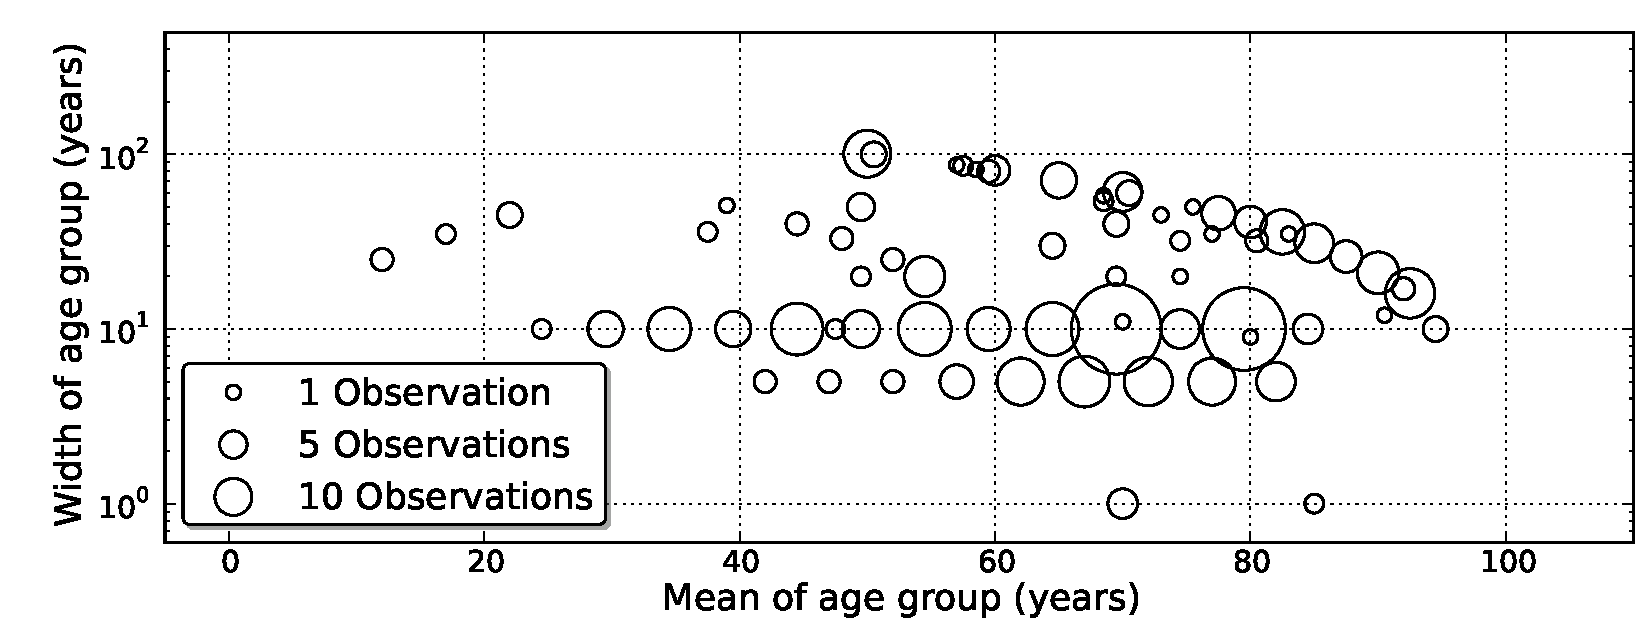
\includegraphics[width=\textwidth]{af_age_groups_scatter.pdf}
%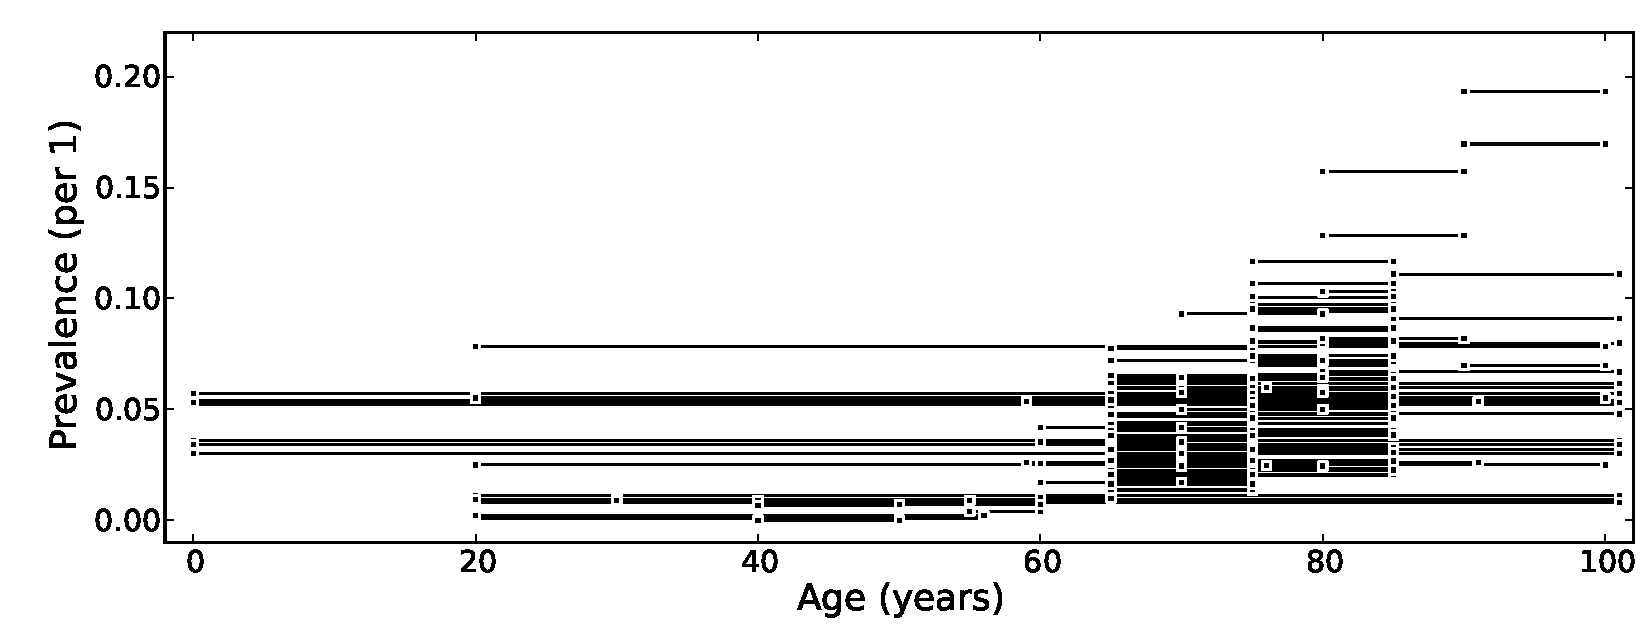
\includegraphics[width=\textwidth]{af_ages_intervals.pdf}
\end{center}
\caption{Mean and spread of age groups in the prevalence data
  collected from a systematic review of atrial fibrillation. The
  size of the circle shows how many observations of this age group
  were found in systematic review. There were
  $586$ rows of prevalence data
  extracted, but the most common age group accounted for only
  $68$ rows.}
\label{age-group-model-af-age-groups}
\end{figure}

This variation in reporting would not be problematic if I had access
to the microdata from all the systematic review studies.  For
example, using microdata from a national health information system or
from a demographic household survey, I could simply tally the
prevalence rates by single-year age groups.  Although each individual
rate gathered in this way would have high variability, the rate model
from chapter~\ref{theory-rate_model} combined with the spline model
for an age-specific hazard function from chapter~\ref{theory-age_pattern_model} would
work together to produce an estimate that is as uncertain as it should be.

Although reanalysis from microdata is occasionally implemented in a GBD study,
it is often not an option.  I expect microdata
reanalysis to become more frequent in national and subnational
settings.  In the more common situation where rate microdata are not
available, the rates cannot be retallied into homogeneous age groups,
and an alternative approach is needed.

This setting is in some ways similar to the settings where interval
regression methods are applied in
econometrics.\cite{amemiya_regression_1973,manski_inference_2002,cook_partially_2012}
However, the econometric approach assumes only that the covariate
value is known to be between upper and lower bounds, while I have more
information about the structure of the data that I can leverage in my
model.

I have considered several statistical approaches, and
they will be compared and contrasted in this chapter.  Before getting
into the details, however, it is worthwhile to examine theoretically
the way that age-grouping functions.

I begin with a simple mechanistic model of the age-grouping process.
A study conducts some sort of measurement on a population of
individuals who are all of different ages, and then the
epidemiological rate or rates of interest are tallied for age groups
selected in some context-dependent manner. If the study was a
prevalence study using a full census sample, for example, and if I use
$r_{a_0,a_1}$ to denote the rate for age group $(a_0, a_1)$ and
$n_{a_0,a_1}$ to denote the subpopulation size of age group
$(a_0,a_1)$, then the identity
\[
n_{a_0, a_2} = n_{a_0,a_1} + n_{a_1,a_2}
\]
says nothing more complicated than that the size of the subpopulation
of age at least $a_0$ and less than $a_2$ is the sum of the size of
the subpopulation between ages $a_0$ and $a_1$ and the size of the
subpopulation between ages $a_1$ and $a_2$.  Applying the same
observation to the parts of these subpopulations that have the condition
of interest yields the following identity:
\[
r_{a_0,a_2} = r_{a_0,a_1}\frac{n_{a_0,a_1}}{n_{a_0,a_2}} + r_{a_1,a_2}\frac{n_{a_1,a_2}}{n_{a_0,a_2}}.
\]
In a limiting case of a very large population with very fine age
intervals, this becomes
\[
r_{a_0,a_2} = \int_{a=a_0}^{a_2} r_{a,a+\d a}\frac{n_{a,a+\d a}}{n_{a_0,a_2}}\d a.
\]
Undoubtedly, all real studies are more complicated than this full
census of prevalence, but this is a starting point for conceptualizing
where age-grouped rates come from.  Roughly, they are integrals over
instantaneous rates for infinitesimal age groups.

\section{Overlapping age-group data}
\label{theory-age_group_model-overlapping_data}
This section uses graphical statistics to explore an example of overlapping age-group data
collected in systematic review.  The
primary way I like to display overlapping age-group data with horizontal
lines on a plot of age versus rate value, as shown in
figure~\ref{theory-age_group_model-dismod_data_plot}.  The level of the bars shows
the rate value, while the width of the bars shows the range of ages
included in the age group. It is often informative to augment these
lines with error bars that show the uncertainty reported for each rate
value, but for this section I have left out the representation of
uncertainty to keep the plots as simple as possible.

\begin{figure}[ht]
\begin{center}
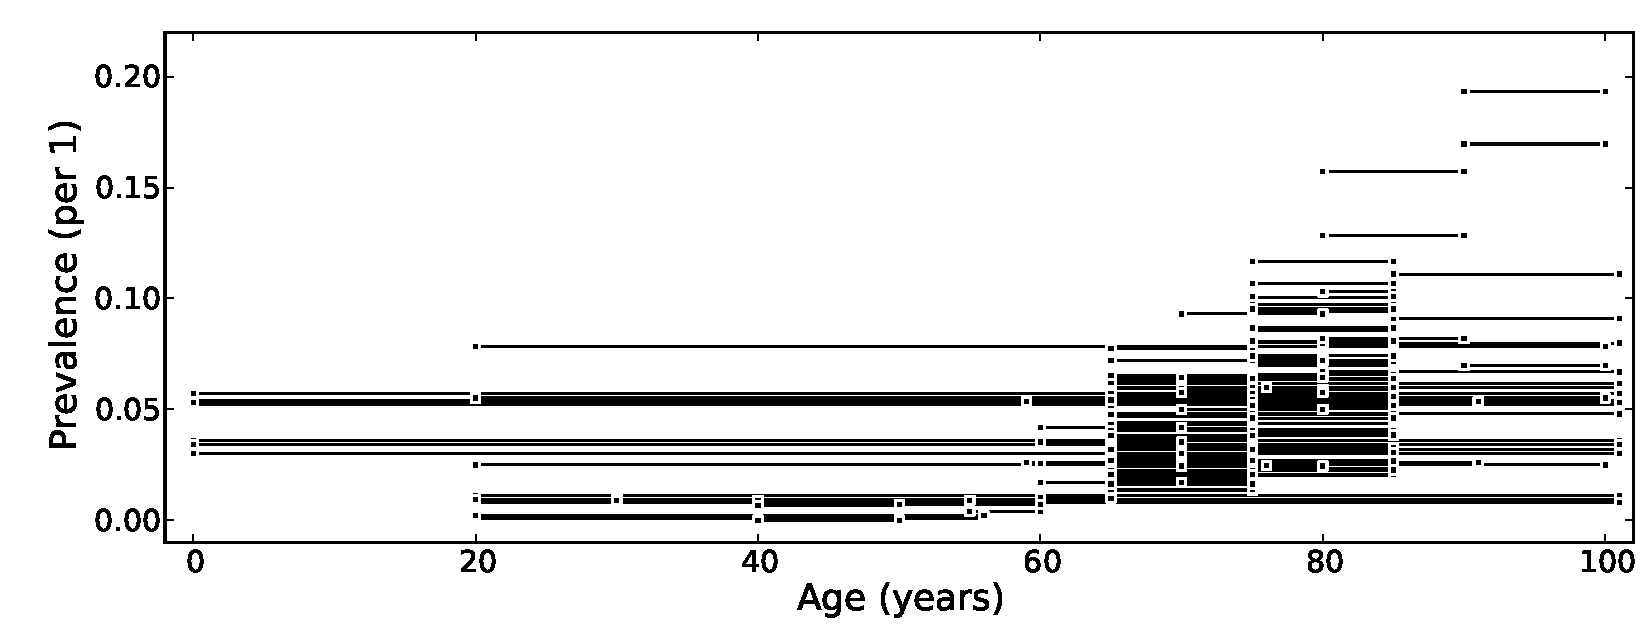
\includegraphics[width=\textwidth]{af_ages_intervals.pdf}
\caption{The systematic review of the descriptive epidemiology of
  atrial fibrillation included $155$ observations of disease prevalence for the United States.
 The prevalence level and age group of
  each observation are shown as a horizontal bar, with the
  position of the bar along the $y$-axis representing the prevalence
  level and the endpoints along the $x$-axis representing the start and
  end of the age group.  The data show heterogeneity by age that is
  typical for these systematic review results and that clearly increases
 with age.  }
\label{theory-age_group_model-dismod_data_plot}
\end{center}
\end{figure}

Each of the horizontal lines in
figure~\ref{theory-age_group_model-dismod_data_plot} can be
represented as a triple $({a_s}, {a_e}, r)$, where $a_s$ is the
starting age of the age group, $a_e$ is the ending age of the
age group, and $r$ is the rate observed for this age group.

A brief word about ${a_e}$ is in order here.  Often in the
epidemiological literature, the ending ages are described in a
unit-dependent fashion, for example, age group $10$--$14$.  This is intended
to mean from the first day of age 10 to the last day of age $14$.
However, this notation can be a hindrance when dealing with age
resolution finer than $1$ year, a situation that comes up when studying
neonatal conditions.  For this reason, I prefer the approach that
takes the end age of the interval to be the first age when an
individual is no longer part of the group.  In the case above, I would
say ${a_e} = 15$.


With a firm understanding of the sort of overlapping age-group data
that arise in systematic review, I now turn to developing and
analyzing a series of models for the meta-analysis of the data.
I will consider five: the midpoint model, the disaggregation
model, the midpoint-with-covariate model, the age-standardizing model,
and the age-integrating model.  The age-standardizing model is the
balance of theoretical foundations, practical implementability, and
empirical success that is used in the second half of this
book.

\section{Midpoint model}
\label{theory-age_group_model-mp_model}
The simplest approach to modeling data with heterogeneous age
intervals is to apply each rate measurement to the midpoint of the
age group it measures.  This is trivial operationally, but it is also
theoretically justified through a ``trapezoidal rule'' integration.

In practice, this approach is quite accurate for modeling a
disease rate that changes slowly as a function of age.  However, it
becomes inaccurate when modeling rates change more
rapidly.  The typical setting in applications in the second half of
this book will include both a few studies that focus on age patterns and
hence have narrow age groups and also many studies
that focus on other aspects of disease epidemiology.  Thus, when
considering how these models are inaccurate, the relevant setting is where
there are a few small age-group studies and many large age-group
studies.

Mathematically, the formulation is as follows: let $h(a)$ be a
process model for the age-specific function (e.g., a spline model
from chapter~\ref{theory-age_pattern_model} or the age-specific prevalence function derived from the solution to the system of differential equations from section~\ref{sys-dynamics}), and let $\dens(r,n\given
\mu,\rho)$ be a data model for the observed level (e.g., the probability
density function for the negative-binomial rate model from
chapter~\ref{theory-rate_model}).
Then the likelihood of an observation of rate $r_i$ with effective
sample size $n_i$ for age group $({a_s}_i, {a_e}_i)$ is simply
$\dens\left(r_i, n_i \given h\left(\frac{{a_s}_i+{a_e}_i}{2}\right),
\rho\right)$. Equivalently, in ``blackboard notation,'' using
$\scD(\mu, \rho; n_i)$ to denote the rate model distribution, I can
write
\begin{align*}
r_i &\sim \scD\left(h(a_i), \rho; n_i\right),\\
a_i &= \frac{{a_s}_i+{a_e}_i}{2}.
\end{align*}
This formulation will be convenient for comparison with the other models of age groups to come.

To understand how accurately age-group models like the midpoint model
can estimate, I used simulation.  The precise details are deferred
until section~\ref{agm-compare}, but since this simulation is also used for the
figures that follow, I will describe it briefly here.  First, I
selected an age-specific hazard function as ground truth.  Then I
generated noisy measurements from a mixture of regularly spaced
$10$-year age groups and uniformly random age groups.  For each
measurement, I chose a random population structure and integrated the
true age-specific hazard to find the true rate for the age group.
Then I sampled from a negative-binomial distribution with this true
rate as the mean and a fixed overdispersion parameter to obtain noisy
data, which I used in the age-group model.  Since ground truth is
known in this simulation, I can compare the model estimates to the
truth graphically as well as quantitatively.

Figure~\ref{midpoint} compares the estimate produced by the midpoint
model to ground truth through simulation using two different
age-specific hazard functions as ground truth.  When the age-specific
hazard varies little as a function of age, as shown in panel (a), the
estimated hazard function is quite accurate.  But when the age-specific hazard function
varies substantially, as shown in panel (b), the estimate is biased.


\begin{figure}[h]
\begin{center}
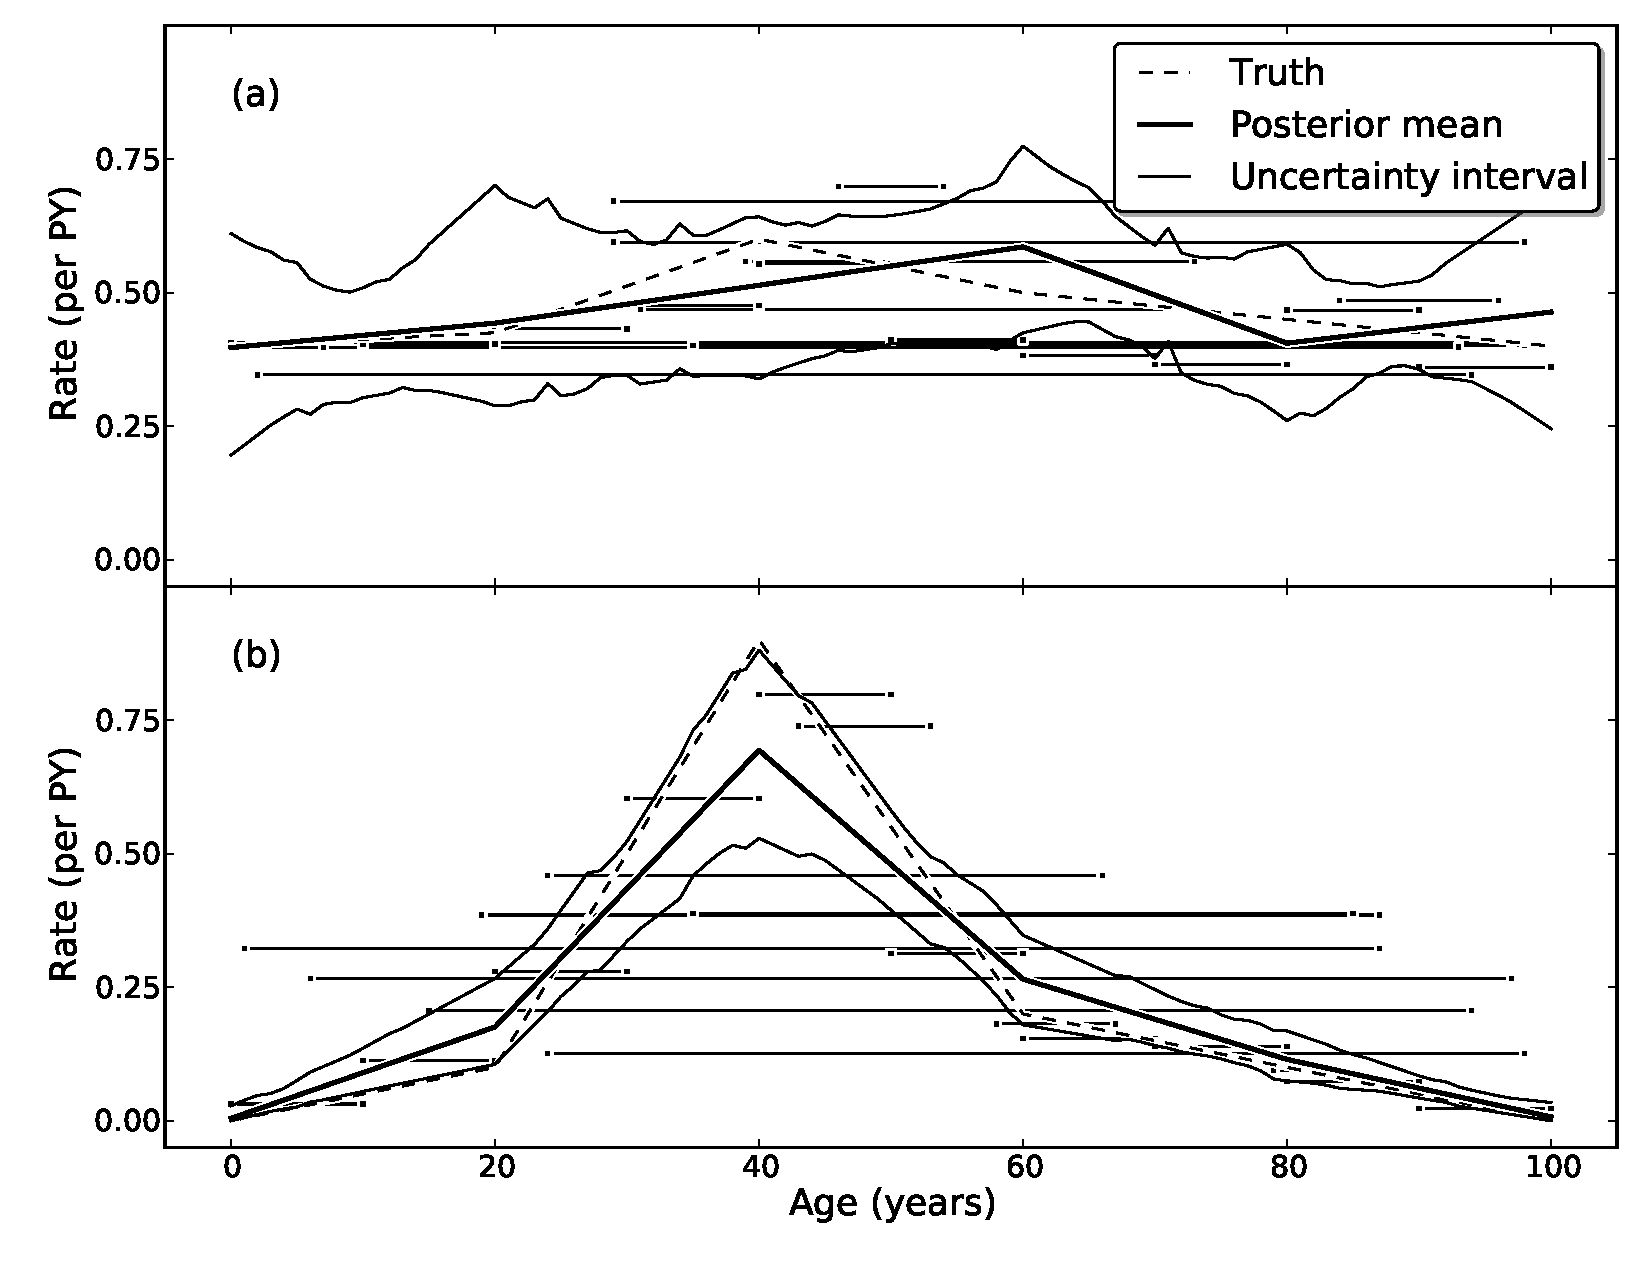
\includegraphics[width=\textwidth]{age_group_midpoint.pdf}
\caption{The midpoint model, a conceptually simple approach to
  dealing with data with heterogeneous age groups, simply
  attributes the observation to the midpoint of the age group.  Panel
  (a) shows the model applied to an age-specific hazard function that does not
  vary a great deal across ages; the midpoint model is an
  accurate fit.  Panel (b) shows the model applied to a more variable age-specific hazard function;
  the midpoint model overcompresses the
  estimates.}
\label{midpoint}
\end{center}
\end{figure}


\section{Disaggregation model}
An alternative to the midpoint model that seems appealing but has
some downsides is what I call \emph{disaggregation}.  To understand
the disaggregation approach, imagine the simple reanalysis that I
could do if microdata were available (as described at the beginning of
this chapter).  If I had access to the individual measurements that
went into the calculation of the disease rate found in systematic
review, I could do a reanalysis with any age grouping I wished. I
could calculate rates for single-year age groups and be sure that the
age pattern does not change substantially during the grouping.

The microdata from rates found in systematic review are rarely
available, however. The disaggregation approach is a simple attempt to
impute what the rates for the desired age grouping would be \emph{if}
the microdata were available. This requires taking into account the
increased variation that would be found if a study of the same size
was reported for finer age groups.

Without any additional information, rate data reporting a level of $r$
for a population with effective sample size $n$ for age group $(a_s,a_e)$, that is,
\[
X = (r, n, a_s, a_e)
\]
can be disaggregated into $A = a_e-a_s$ rows of
data, $X_1, X_2, \ldots, X_A$, with
\[
X_a = \left(r, \frac{n}{a_e-a_s}, a, a+1\right), \text{for } a=1,2,\ldots,A.
\]

Disaggregation can be interpreted as a data-preprocessing step, and
these disaggregated data can be fed into the midpoint model from the
previous section to produce a comprehensive estimate of the rate as a
function of age. However, this model has some unintended negative
features when large age intervals are disaggregated.  Because it
ignores the correlation of disease levels with age, it tends to
overcompress age patterns at young and old ages, as shown with simulated data in figure~\ref{disagg}.

\begin{figure}[h]
\begin{center}
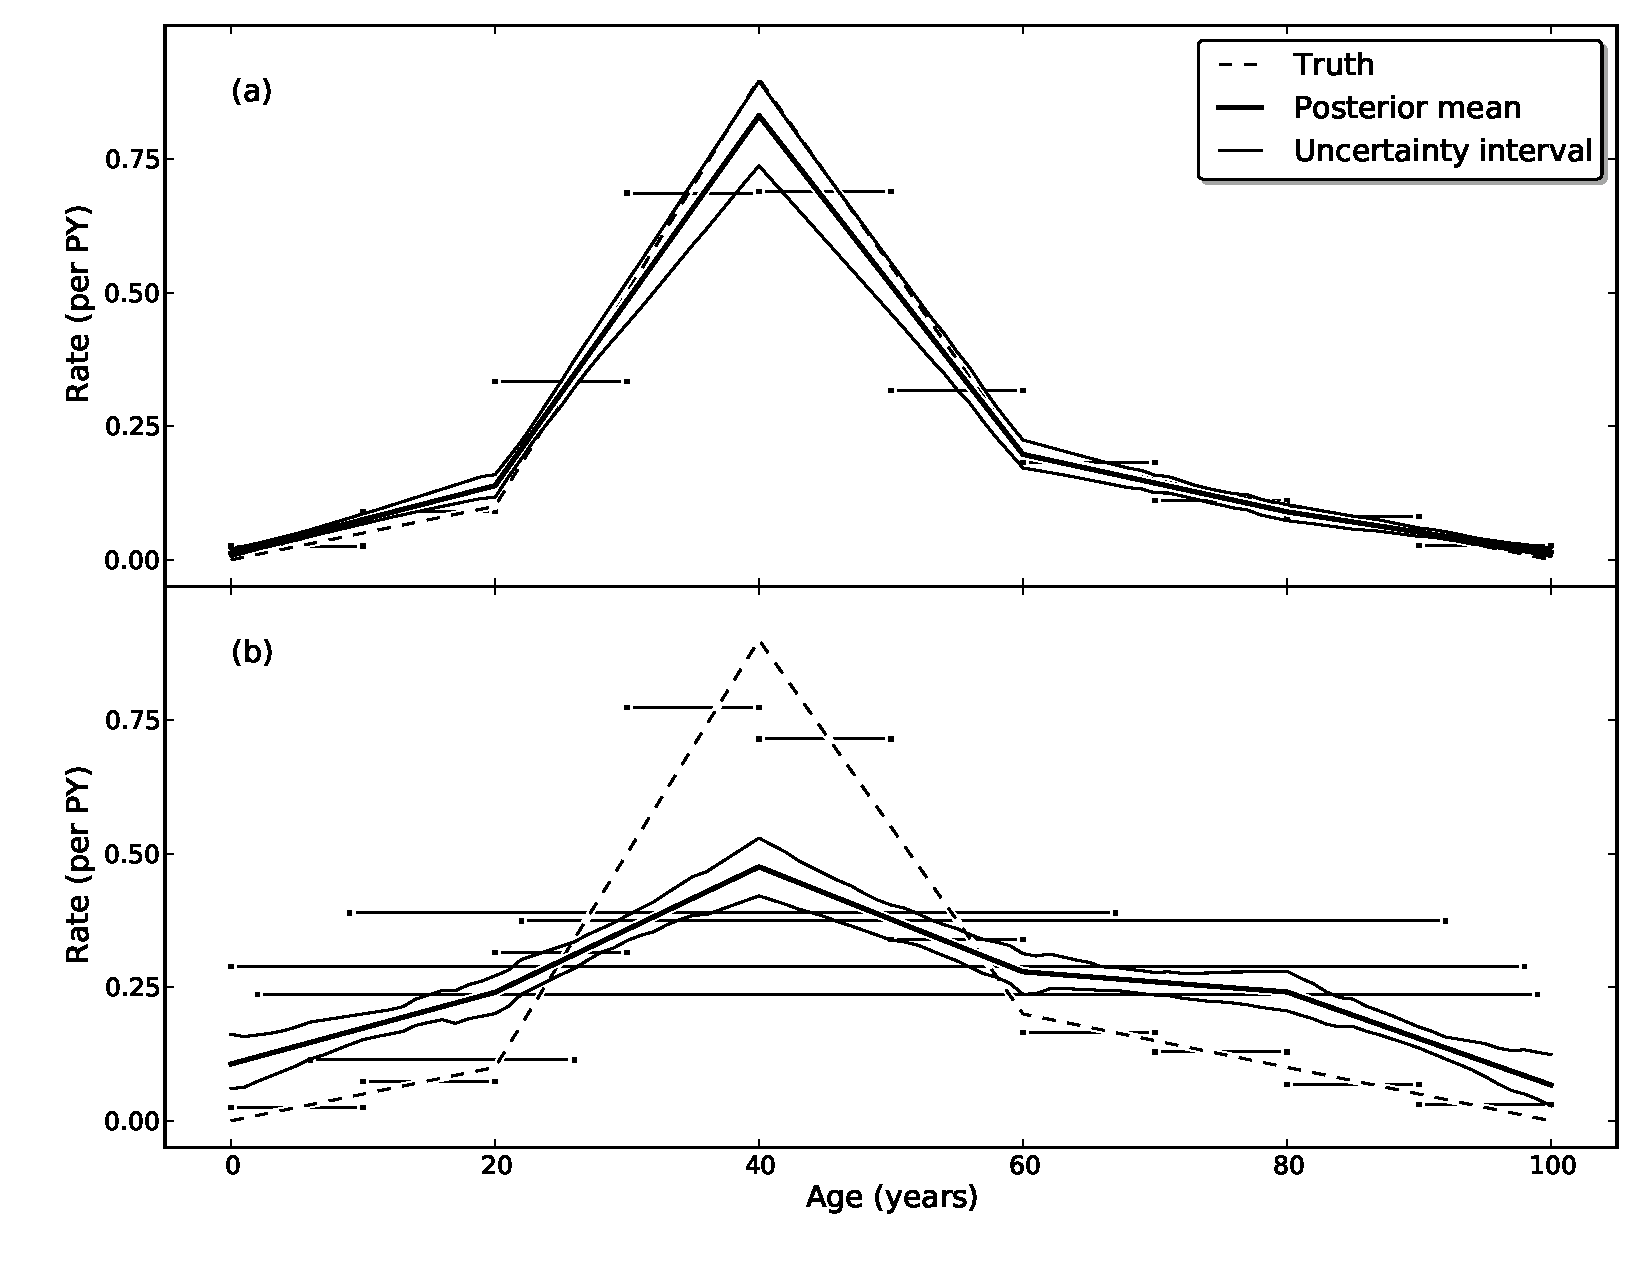
\includegraphics[width=\textwidth]{age_group_disagg.pdf}
\caption{This figure shows the effects of fitting a model with my
  disaggregation approach to two simulated data sets.  When the age groups are sufficiently
  fine-grained and homogeneous, disaggregation is a successful
  approach.  But with even slight heterogeneity, as in panel (b), the model
  estimates are overcompressed.}
\label{disagg}
\end{center}
\end{figure}


\section{Midpoint model with group width covariate}
An alternative method, which I consider more ``statistical'' in its
approach, is to add the width of the age group as a covariate into the
midpoint model.  This model takes the form
\begin{align*}
r_i &\sim \scD\left(\mu_i, \rho; n_i\right),\\
\mu_i &= h\left(\frac{{a_s}_i+{a_e}_i}{2}\right) + \theta (a_e - a_s).
\end{align*}

This addresses the shortcomings of the disaggregation approach
\emph{indirectly}, and the indirect nature has positives and
negatives.  This method does not explicitly connect the large age
interval to the small age interval but instead allows the data to
inform the relationship.  On the other hand, it posits that the
data-driven relationship between the rates for studies with the same
midpoint but different age groups is a linear relationship. In
contrast, the mathematical model developed at the beginning of this
chapter is nonlinear in
a specific and mechanistically known way.
Figure~\ref{midpoint-covariate} shows the results of applying the midpoint-covariate
model to simulated data.


\begin{figure}[h]
\begin{center}
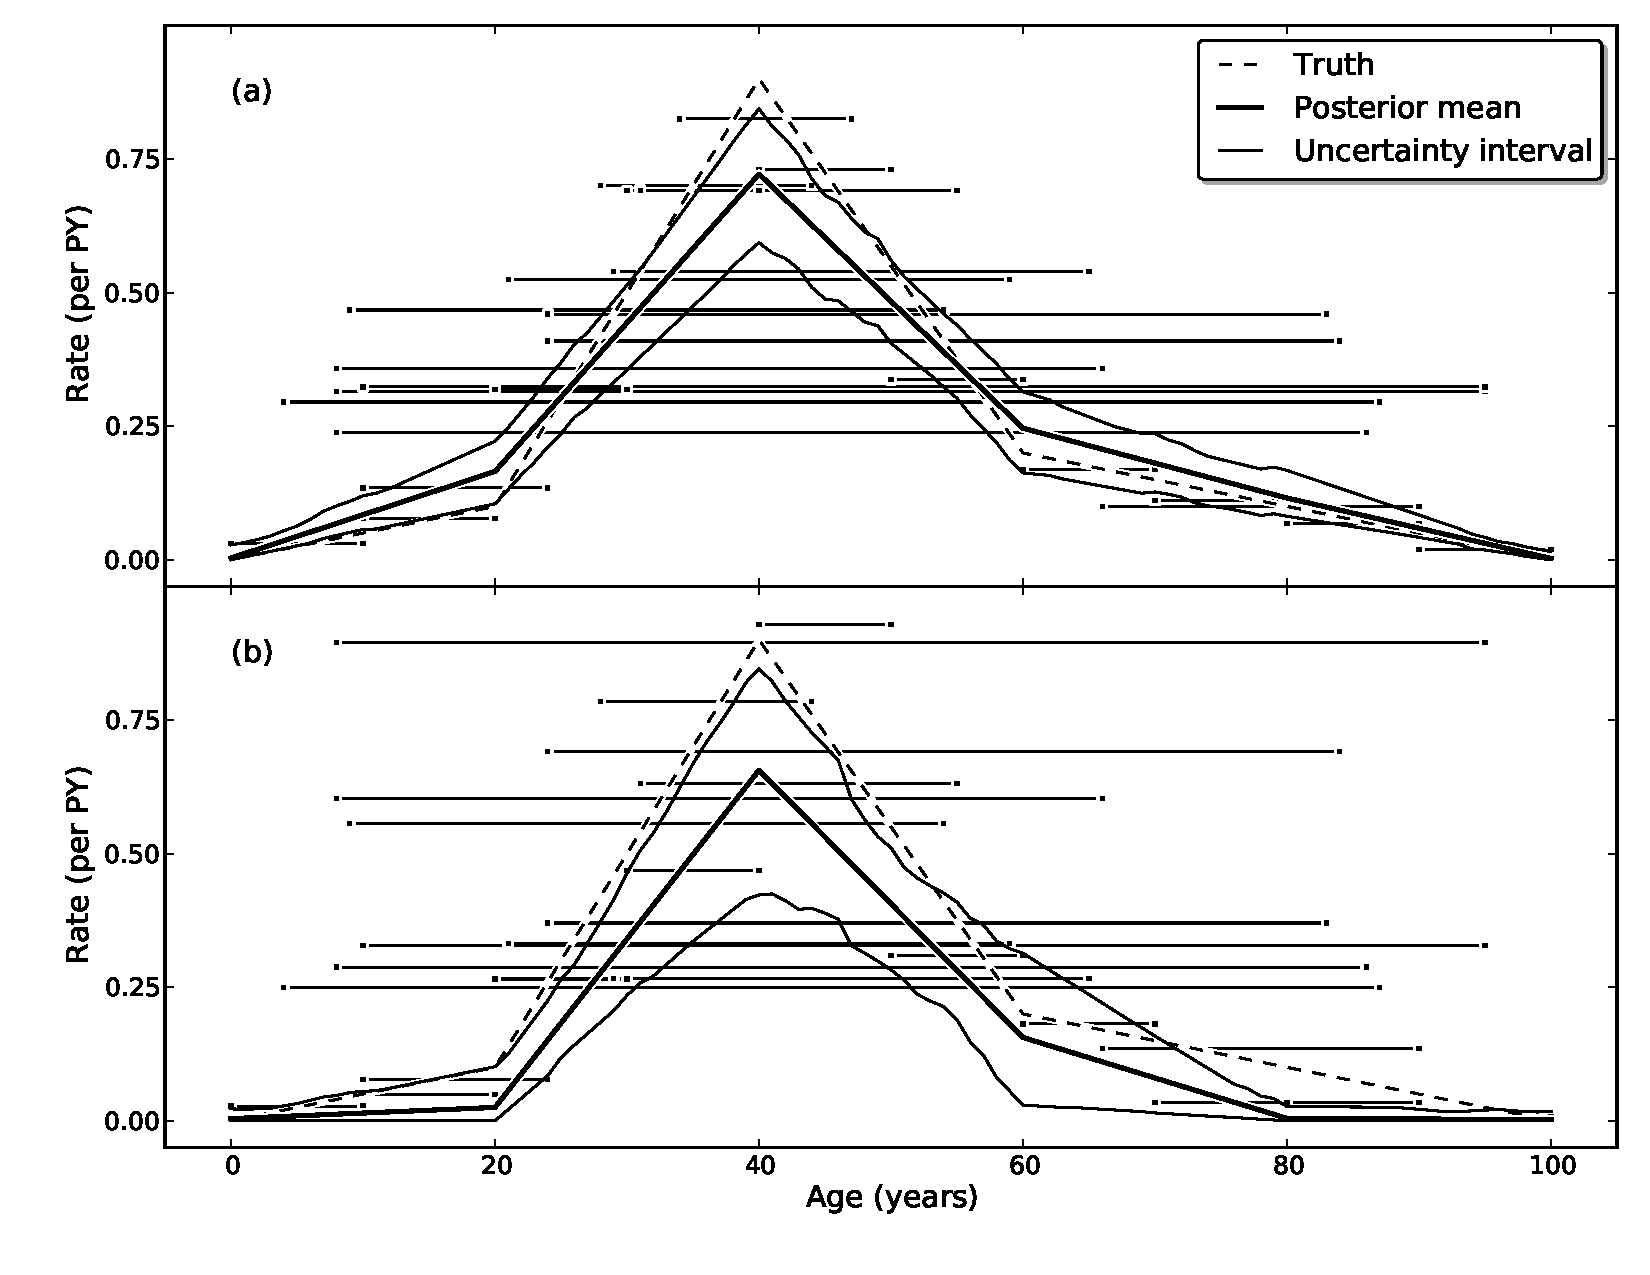
\includegraphics[width=\textwidth]{age_group_midpoint_covariate.pdf}
\caption{The midpoint-covariate model applied to two simulated
  data sets, where ground truth is known. Although this approach is
  appealing theoretically, the added flexibility of the covariate
  model does not add much value in the simulation study. }
\label{midpoint-covariate}
\end{center}
\end{figure}

\section{Age-standardizing and age-integrating models}
\label{age-standardizing}
An even more complicated approach, both conceptually and
computationally, is to average across the age interval explicitly in
the statistical model:
\begin{align*}
r_i &\sim \scD\left(\mu_i, \rho; n_i\right),\\
\mu_i &= \int_{a={a_s}_i}^{{a_e}_i} h(a)\d w_i(a),
\end{align*}
where the integration $\d w_i$ is weighted according to population
structure.

This has the theoretical appeal of matching the generative model above
but the drawback of being slower computationally and less stable
numerically.  It also has a major piece left unspecified: the
selection of the age weights for the integration.  There are two
sensible approaches to rectifying these shortcomings, which I call the \emph{age-standardizing
  model} and the \emph{age-integrating model}.  The age-standardizing
model uses a common age pattern $\d w_i(a) = \d w(a)$ for all studies, while
the age-integrating model uses the best estimate available of the age
pattern of the study population in each observation.  The
age-standardizing model is faster, due to a computational optimization
only possible when the $\d w_i$ are the same for all $i$, but the
age-integrating model is appealing on theoretical grounds, because it
can use more information.  However, it is not certain that
using this information will make the end results any more accurate,
because the age pattern of the study population is rarely known with
much certainty, and often it is necessary to assume that it matches
the national age pattern for the country-years where the study was
conducted.  In the case of remission and mortality studies it is even
more complicated to estimate the study population age pattern, since
it is \emph{not} the same as the national population age pattern but
modulated by the age pattern of disease prevalence.
Figure~\ref{age-group-standardize} shows the results of the age-standardizing model on
simulated data.

\begin{figure}[h]
\begin{center}
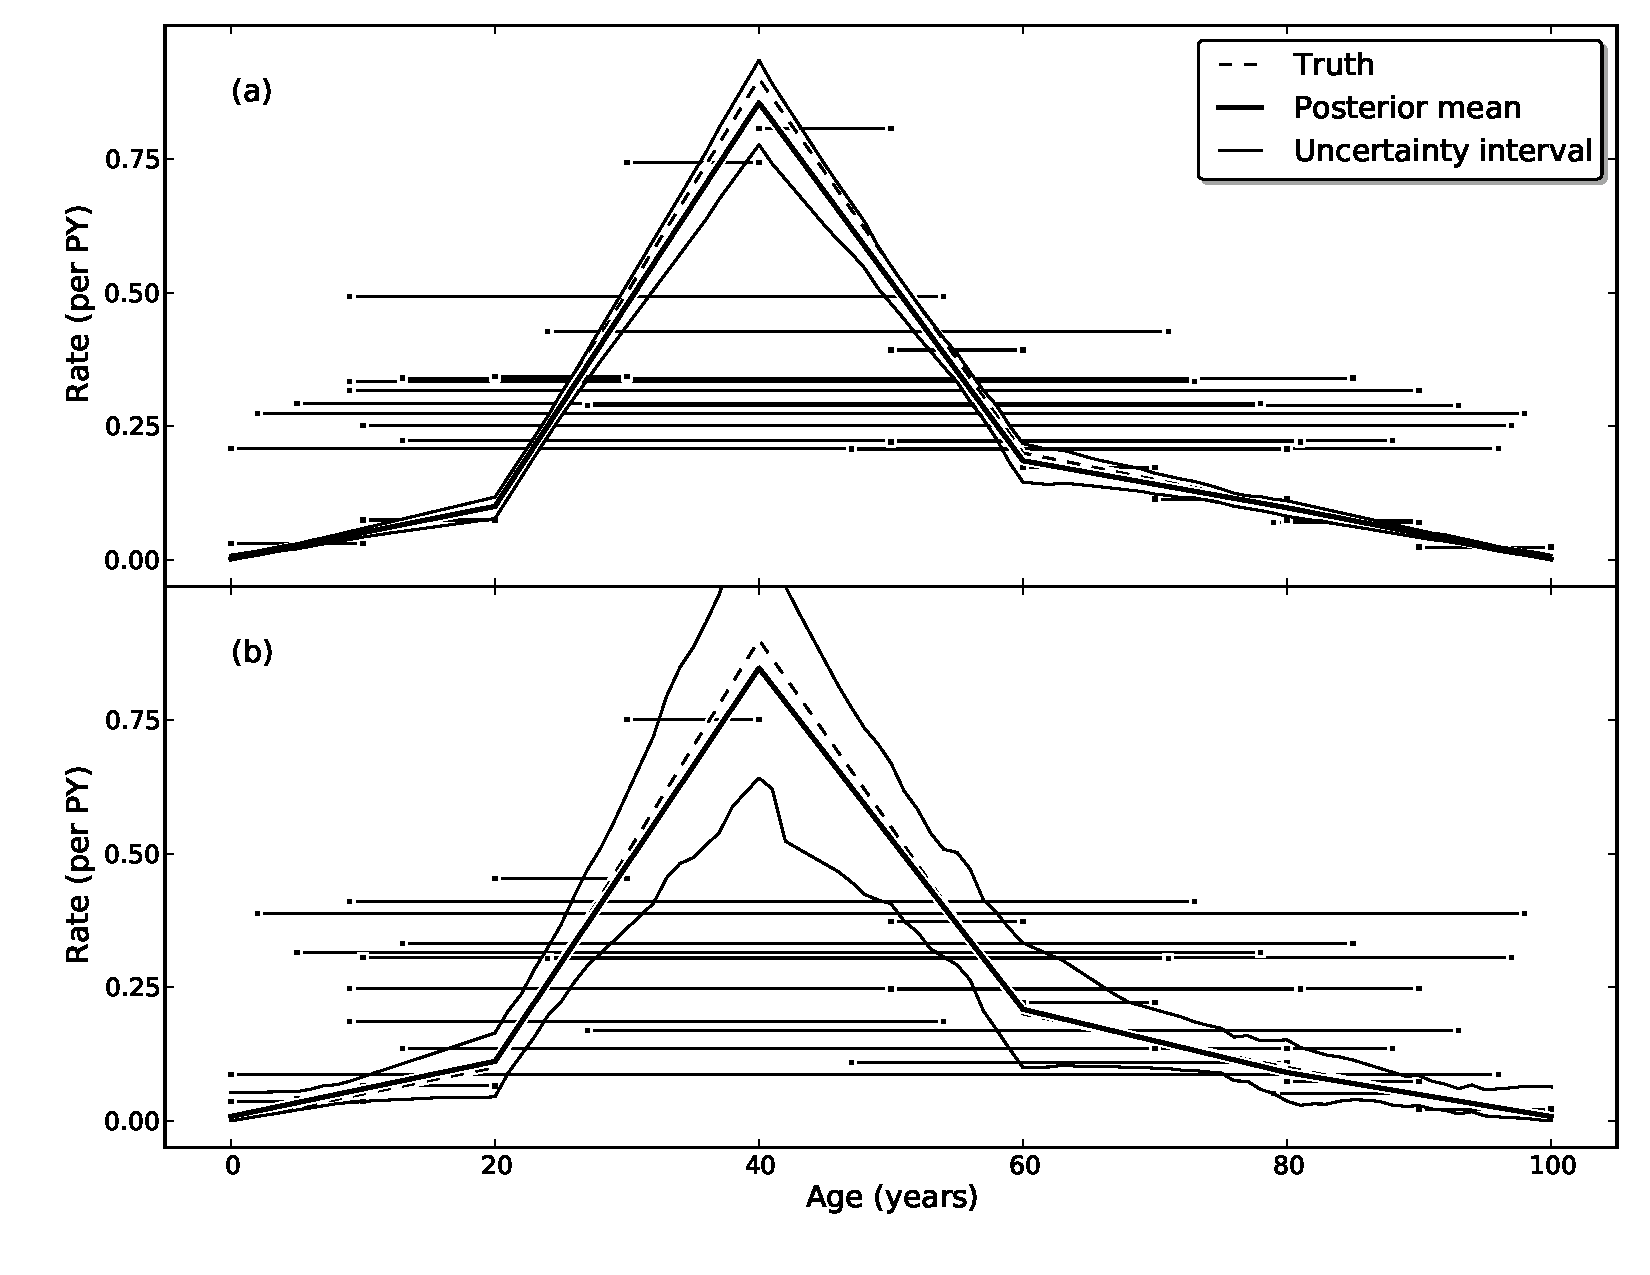
\includegraphics[width=\textwidth]{age_group_standardize.pdf}
\caption{The age-standardizing model applied to simulated data with a
  known age-specific rate function as ground truth.  The results in
  panel (a) show that the model
  recovers the true age pattern quite precisely. Panel (b) shows that the
  results are still accurate when the data generation procedure is
  even more noisy.}
\label{age-group-standardize}
\end{center}
\end{figure}


\section{Model comparison}
\label{agm-compare}

\begin{figure}[h]
\begin{center}
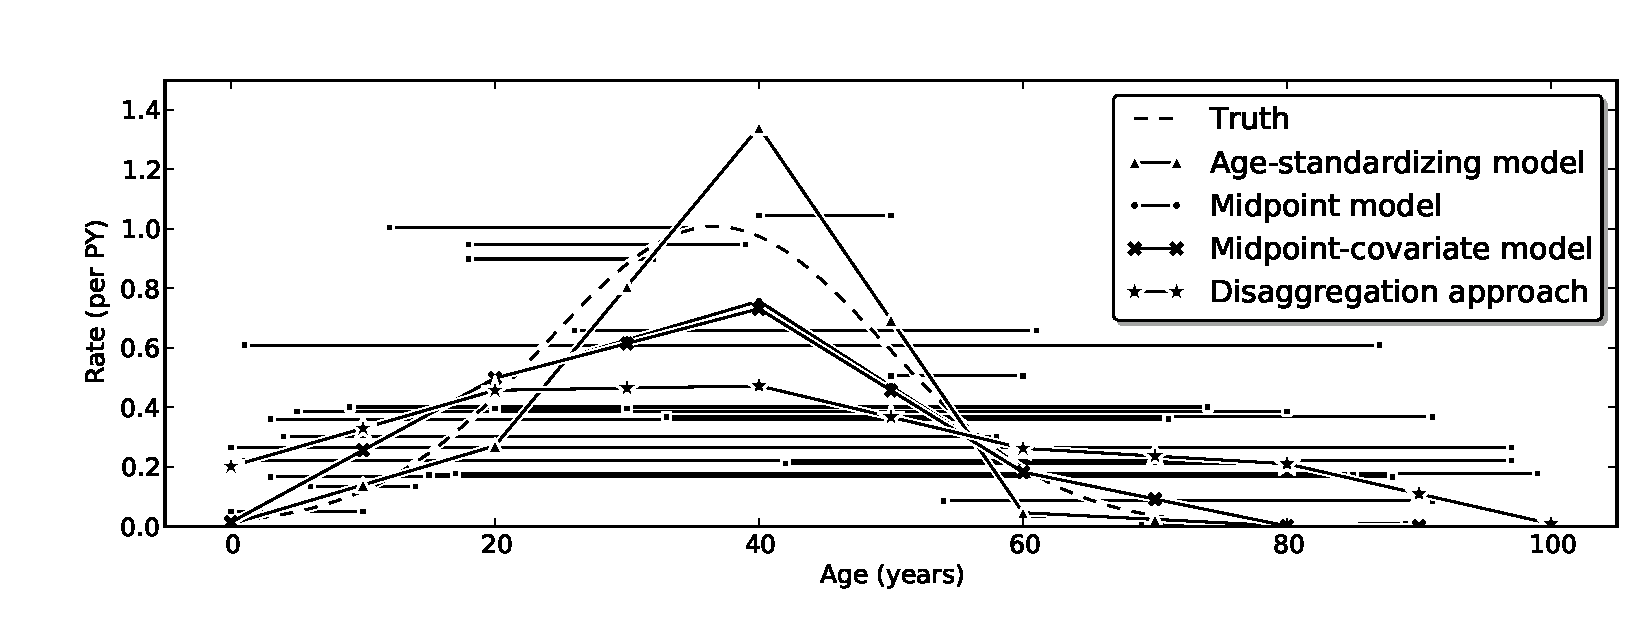
\includegraphics[width=\textwidth]{age_group_models.pdf}
\caption{A comparison of $4$ models for heterogeneous age groups shows that the age-standardizing model comes closest to recovering the truth.  This corresponds to the results of the simulation study presented in table~\ref{age_group_comparison}.}
\label{age-group-model-comparison}
\end{center}
\end{figure}


This section provides a comparison of the approaches to age-group
modeling.  An appropriate comparison of these approaches is somewhat difficult to
develop.  One approach is through simulation, where a data set is
simulated from known ground truth (figure~\ref{age-group-model-comparison}).
This allows the estimates to be
compared to ``true'' values, but this risks
inappropriate model selection due to inaccurately choosing the
distribution of the simulated data.  Another approach is
cross-validation, where data from systematic review are split into
mutually exclusive
\emph{training} and \emph{test} sets, and the model is fitted to the
training set and used to predict the values in the test set.  Naively
holding out $25\%$ of the data does not address the exact topic of
interest, however, since it determines which model predicts rates of
all age groups, and I am really only interested in predicting the age groups
with small widths accurately.  It would be preferable to hold
out only data with small-width age groups from large representative
subpopulations.  Unfortunately, there are rarely enough data to do this,
especially in all the settings that come up in disease modeling.

I have taken a pragmatic approach, evaluating by means of the natural
simulation described below.  Future work, based on more sophisticated
simulation scenarios or based on carefully designed holdout
cross-validation, is necessary to further understand the trade-offs
between these alternative methods.

The data simulation procedure I used is the following:
\begin{itemize}
\item Choose age intervals for $30$ rows of data; for $i=1,\ldots,10$,
  $({a_s}_i,{a_e}_i) = (10(i-1), 10i)$, and for the remaining $20$
  intervals, choose the age interval width uniformly at random from $[1,100]$
  and choose the midpoint of the age interval uniformly at random from ages
  within this age range.

\item Choose the effective sample size $n_i$ for each row uniformly at random from $[10^2, 10^4]$.

\item Choose an age-specific population structure for each row of data,
  with the form $w_i(a) = e^{\beta_i a}$, where $\beta_i$ is drawn
  from a normal distribution with mean $0$ and standard deviation
  $\frac{1}{10}$.

\item Calculate the true rate value for each age interval,
  \[ r^\text{true}_i = \sum_{a={a_s}_i}^{{a_e}_i} \mu_\text{true}(a)
  w_i(a),\] where \[ \mu_\text{true}(a) =
  \exp\left(\frac{3(a-35)^2}{1000} + \frac{a-35}{100}\right). \]

\item Choose an observed rate value, based on a negative binomial distribution:
$r_in_i \sim \NegativeBinomial(r^\text{true}_i, \delta_\text{true})$, where $\delta_\text{true} = 5$.
\end{itemize}

Table~\ref{age_group_comparison} shows the median results of fitting this simulated data for a variety of models. The age-standardizing and age-integrating models are
superior in all metrics of fit quality.  The age-standardizing
model has a computation time that is only slightly longer than the fastest approach,
while the age-integrating model is $26\%$ slower.

\begin{table}

\begin{center}
\begin{tabular}{|c|c|c|c|c|}
\hline
Model&Bias (\%)&MAE (\%)&PC (\%)&Time (s)\\
\hline
Midpoint&0.02&0.08&0.8&29.0\\
Disaggregation&0.03&0.19&0.08&52.6\\
Midpoint-covariate&0.03&0.09&0.89&45.8\\
Age-standardizing&0.01&0.04&0.95&30.3\\
Age-integrating&-0.0&0.03&0.78&38.1\\
\hline
\end{tabular}
\end{center}

\caption{Median results for $100$ replicates of the simulation study
  comparing age-specific rate estimates from $5$ models of age-grouped
  data, showing bias (mean of true minus predicted), median absolute
  error (mae, median of absolute difference between truth and
  predicted), probability of coverage (pc, fraction of truth falling
  within 95\% uncertainty interval of prediction), and computation time. }
\label{age_group_comparison}
\end{table}
